\chapter{第九關:指標}

%L9_01 梁A047
\section{不定數排序--插入排序法}
\label{L9_01}
輸入一個數字n,後面接著n個數字,將這n數從小印到大。

\subsection{解題思維}

這個題目希望我們使用插入排序法處理,所以先介紹插入排序法的概念。
想像我們在玩撲克牌的時候,要把牌子從小排到大,
假設有$n$張牌都已經排序好了,現在加入一張牌,我們會直接找看看
這張牌應該插入在哪裡,這樣就完成了$n+1$張的排序。
依照這樣的方法,每次加入一張排序,就可以把整個數列排好。

更具體來描述,可以將演算法說明條列如下:
\begin{enumerate}
	\item 將數列區分為兩組,左邊$i$個已排序,右邊未排序。
	\item 取第$i+1$個數當作處理值。
	\item 在$i$個已排序的數列中,找到適合第$i+1$個數的位置(可以從前面找起,或者從後面找起),假設位置為$k$,
	將$k$之後的數都往後移一格,並將處理值放在位置$k$。
	\item 已排序的數列長度加1,重複以上步驟,直到全部的數都排序完畢。
	\begin{figure}[H]
		\centering
		\includegraphics[width=0.3\textwidth]{fig/L9/L9_01}
		\caption{插入排序法示意圖}
	\end{figure}
\end{enumerate}

一般在處理第三個步驟時,通常希望使用 in-place 方式處理,也就是改變原先的陣列來達成。
這有許多方式可以達成,例如,我們可以先把要處理的值存起來,假設其值為 $p$,
接下來從已排序的數列中的最後一個值找起,只要比 $p$ 大,就將其往後移一格。
直到找到一個小於或等於 $p$ 的數,或則已經找到 -1 的位置(已超出陣列),這時就在這個位置的後面插入 $p$。

使用這樣的方式其演算法可以描述如下:
\begin{inside}
	for (i=0; i<n; i++) { // 假設i以前已處理好,i是要處理的位置
		p = a[i]; // 先把a[i]存起來,以免被蓋掉
		for (j=i-1; j>=0 && a[j]>p; j--) { // 位置小於等於0,且值比p大
			a[j+1] = a[j]; // 把j位置的數移到j+1
		}
		a[j+1] = p; // 在找到的位置後面放p
	}
\end{inside} 

以下在瘋狂程設接連的幾題插入排序法,要求不能出現數字$1\sim 9$,
這樣的話,我們要做一點調整,讓$1\sim 9$不要出現。
基本上這也有很多做法,以下僅提供一個簡單的想法。
\begin{inside}
	for (i=0; i<n; i++) { // 假設i以前已處理好,i是要處理的位置
		p = a[i]; // 先把a[i]存起來,以免被蓋掉
		k = j = i; // k和j都設成i
		for (j--; j>=0 && a[j]>p; ) { // 位置小於等於0,且值比p大
			a[k--] = a[j--]; // 把j位置的數移到k,之後j和k各減1
		}
		a[k] = p; // 在找到的位置後面放p
	}
\end{inside} 

有了以上的了解之後,這個題目就不難解答了。

首先是處理輸入的問題,題目說輸入n,之後再接著n個數,再把這n個數從小排到大。
那這樣的話,我們可以先讀入n之後,再來宣告一個
n個數的陣列(gcc可以接受這樣的方式),
之後把n個數讀入陣列之中,讀完之後,最後再使用我們上面的
插入排序法來排序就可以了。

完整程式碼如下:

\begin{cppcode}
#include <iostream>

using namespace std;

int main()
{
	int n;  cin >> n;
	int a[n];
	for (int i=0; i<n; i++) cin >> a[i];
	for (i=0; i<n; i++) { // 假設i以前已處理好,i是要處理的位置
		int j, k, p = a[i]; // 先把a[i]存起來,以免被蓋掉
		k = j = i; // k和j都設成i
		for (j--; j>=0 && a[j]>p; ) { // 位置小於等於0,且值比p大
			a[k--] = a[j--]; // 把j位置的數移到k,之後j和k各減1
		}
		a[k] = p; // 在找到的位置後面放p
	}
	for (int i=0; i<n; i++) cout << a[i] << " ";
	return 0;
}
\end{cppcode}
 
在處理不定數的輸入時,如果熟悉\cc{}的向量,也可以使用如下的程式碼:
\begin{cppcode}
	#include <iostream>
	#include <vector>
	
	using namespace std;
	
	int main()
	{
		int n, x;
		cin >> n;
		vector<int> v;
		for (int i=0; i<n; i++) {
			cin >> x;
			v.push_back(x);
		}
		for (i=0; i<n; i++) {
			int j, k, p = a[i];
			k = j = i;
			for (j--; j>=0 && a[j]>p; ) a[k--] = a[j--];
			a[k] = p; // 在找到的位置後面放p
		}
		for (int i=0; i<n; i++) cout << v[i] << " ";
		return 0;
	}
\end{cppcode}

另外我們也可以使用動態記憶體配置。

在\cc{}裡面,使用new來配置記憶體空間。像這樣:
\begin{inside}
	int n;  cin >> n;
	int *a = new int[n];
	for (int i=0; i<n; i++) cin >> a[i];
	// 其餘部份同上面程式碼
\end{inside}

在C裡面,使用malloc來配置記憶體空間(要引入stdlib.h)。像這樣:
\begin{inside}
	int n;  scanf("%d", &n);
	int *a = (int*)malloc(sizeof(int)*n);
	for (int i=0; i<n; i++) scanf("%d", a+i);
	// 其餘部份同上面程式碼
\end{inside}


%L9_02 梁 A048
\section{不定數排序--new版}
輸入一個數字n後面接著n個數字,將這n數從小印到大。

\subsection{解題思維}
這題的解題原理,請參照上一題。
此題比較特別的,是規定使用new運算子做動態記憶體配置,另外,
因為限制只能出現一次[,所以除了new運算子使用之外,
其他的a[x]要全部改成 *(a+x)。
最後還有輸出的格式要求,每輸出10個值之後必須換行。

\vspace{0.5cm}
\noindent 程式碼如下:
\subsection{程式碼}
\begin{cppcode}
	#include <iostream>
	
	using namespace std;
	
	int main()
	{
		int n; cin >> n;
		int *a = new int[n];
		for (int i=0; i<n; i++) cin >> *(a+i);
		for (int i=0; i<n; i++) {
			int j, k, p=*(a+i);
			k = j = i;
			for (j--; j>=0 && *(a+j)>p; k--, j--) *(a+k)=*(a+j);
			*(a+k) = p;
		}
		for (int i=0; i<n; i++) {
			if (i>0 && i%10==0) cout << endl;
			cout << *(a+i) << " ";
		}
		delete[] a; // 本題要求出現delete,釋放動態配置之記憶體
		return 0;
	}
\end{cppcode}


%L9_03梁 A049
\section{不定數排序--指標版}
輸入一個數字n後面接著n個數字,將這n數從小印到大。

\subsection{解題思維}
這題的解題原理,請參照上兩題。
此題比較特別的,除了類似上一題的規定之外,
還有以下額外規定:
\begin{enumerate}
	\item 「int n;」 一定要出現一次,
	\item 「int main」 至少出現一次,
	\item 「int」 最多出現兩次,
	\item 「return 0;」 要出現一次,
	\item 「0」 最多出現一次。
\end{enumerate}
不過這一題輸出的時候,不需要每10個數換行。

因為上面的規定,等於其他地方都不可使用int,
也不可使用0,那怎麼辦呢?

讀取數字的部份,如果我們把它改成浮點數,
基本上應該也是OK的,這樣的話,我們可以把
整數陣列改成浮點數陣列。

另外關於0的部份,我們有幾個for迴圈會用到,
譬如讀取的部份,
\begin{inside}
	for (int i=0; i<n; i++) cin >> *(a+n);
\end{inside}

我們可以改用指標來處理,像這樣
\begin{inside}
	for (float *i=a; i<a+n; i++) cin >> *i;
\end{inside}

其他部份的處理也是類似的,這樣的話,我們可以得到
改寫的程式碼如下:
	
\subsection{程式碼}
\begin{cppcode}

#include <iostream>

using namespace std;

int main()
{
	int n; 
	cin >> n;
	float *a = new float[n];
	float p, *k, *j;
	for (float *i=a; i<a+n; i++) cin >> *i;
	for (float *i=a; i<a+n; i++) {
		p=*i;
		k=j=i;
		for (j--; j>=a && *j>p; k--, j--) *k=*j;
		*k = p;
	}
	for (float *i=a; i<a+n; i++) cout << *i << " ";
	delete[] a;
	return 0;
}
\end{cppcode}

%L9_04梁 A050
\section{字串走訪-指標版}
輸入一個連字串,將其印出。

\subsection{解題思維}
\begin{enumerate}
	\item 宣告一個字元陣列,用來儲存字串。
	\item 宣告字元指標p,指向字元陣列。用迴圈印出字串中的每一個字元,當字串結束時,字元陣列會補上一個空字元'$\backslash$0’,該值為false,用來結束迴圈。
\end{enumerate}


\subsection{程式碼}
\begin{cppcode}
	#include <iostream>
	
	using namespace std;
	
	int main()
	{
		char str[1000];
		cin >> str;
		for (char *p=str; *p; p++) cout << *p;
		return 0;
	}	
\end{cppcode}

%L9_05梁 A073
\section{*字元字串-字串長度\underline{ }有問題請勿使用}
輸入一段落,輸出其長度。

\subsection{解題思維}
此題的主程式已經寫好了,我們只需要完成函數STRLEN(char *d)的主體,用來計算字串長度,函數主體的內容如下:
\begin{enumerate}
	\item 函數STRLEN(char *d)的輸入參數是一個地址,可將字元陣列傳入函數中。
	\item 先宣告整數size的初始值為0。
	\item 使用while迴圈,當d[size]有讀到字元,則size++。一直到d[size]的值是是空字元,則結束迴圈。
	\item 回傳size。
\end{enumerate}


\subsection{程式碼}
\begin{cppcode}
	#include <iostream>
	
	using namespace std; 
	
	int STRLEN(char* d)
	{
		// Add your codes here.
		int size=0;
		while (d[size]) size++;
		return size;
	}

	int main()
	{ 
		char d[1024];
		int i;
		for (i=0,cin.read(&d[i],1); d[i]!=10 && d[i]!=13; cin.read(&d[++i],1)); // 讀字元直到換行為止,可改用 gets(d)
		d[i]=0; // 最後設0用來結束字串,用gets則不用
		cout << STRLEN(d);
		return 0;
	} 	
\end{cppcode}

%L9_06 A074
\section{*字元字串-前後字元新增}
完成副程式寫作,在字串前後端新增字元。

\subsection{解題思維}
此題的主程式已經寫好了,我們需要完成函數PUSH\_FRONT(char *d, char c)的主體,用來把字元c插入到字串d的最前面,以及函數PUSH\_BACK(char *d, char c),用來把字元c插入到字串d的最後面。

\vspace{0.3cm}
\begin{enumerate}
	\item 要把字元c插入到字串d的最前面,我們可以將字串d的所有字元,包括最後收尾的0,全部都往後移一格,最後在d[0]的位置填入字元c。移動的順序,可以從最後面開始,才不會蓋到還沒移動的元素。
	\item 要把字元c插入到字串d的最後面,我們只要找到字串d最後收尾的0,然後把該位置改為字元c,並且在後一格的位置填入收尾的0就可以了。
\end{enumerate}


\subsection{程式碼}
\begin{cppcode}
#include <iostream>

using namespace std; 

char* PUSH_FRONT(char *d, char c); // 字串d前面新增字元c
char* PUSH_BACK(char *d,char c); // 字串d最後面新增字元c

int main()
{ 
	char d[1024]; cin >> d; // 輸入字串d
	cout << d << endl;
	cout << PUSH_FRONT(d,'A') << endl;
	cout << PUSH_BACK(d,'Z') << endl;
	return 0;
} 

char* PUSH_FRONT(char*d, char c)
{
	char *p=d; // 設p為字串頭
	while (*p) p++; // 移動p直到字串結尾的0
	for (; p>=d; p--) *(p+1)=*p; // 從最後到頭都往後搬一格
	*d=c; // 第一格設為字元c
	return d;
}

char* PUSH_BACK(char*d, char c)
{
	char *p=d; // 設p為字串頭
	while (*p) p++; // 移動p直到字串結尾的0
	*p++=c; // 最後的0改為字元c,p往後移一格
	*p=0; // 字串最後設0收尾
	return d;
}
\end{cppcode}

%L9_07 A075
\section{*字元字串-前後字元刪除}
完成副程式寫作,在字串前後端刪除字元。

\subsection{解題思維}
此題的主程式已經寫好了,我們需要完成函數POP\_FRONT(char *d)的主體,用來把字串d的最前面字元刪除,以及函數POP\_BACK(char *d),用來把字串d的最後面字元刪除。
另外這題因為題目已經限制解答的部份輸出格式,所以不另外改動程式的排版。

\vspace{0.3cm}
\begin{enumerate}
	\item 要把字串d的最前面的字元移除,我們可以字串d的最前面開始,只要該位置有字元的話,把它的值改成後面的字元,然後再看下一個位置。那如果已經到了字串最後結尾的0,就可以跳出迴圈了。
	\item 要把字串d的最後面的字元移除,我們可以先找到字串d最後收尾的0,然後把它的前一個位置改成字串收尾的0,這樣就刪除該字元了。但必須注意,如果字串長度為0,則不用做任何動作。
\end{enumerate}

\subsection{程式碼}
\begin{cppcode}
#include<iostream>
using namespace std; 
char* POP_FRONT(char*d){
	char*p=d;
	for(;*p;p++)*p=*(p+1);
	return d;
}
char* POP_BACK(char*d){
	if (*d==0) return d; // 空字串直接返回
	char*p=d; // 設p為字串頭
	while(*p)p++; // p遞增直到字串結尾的0
	*(p-1)=0; // 把前一個位置設為0
	return d;
}
int main(){ 
	char d[1024];cin>>d;
	cout<<d<<endl;
	cout<<POP_FRONT(d)<<endl;
	cout<<POP_FRONT(d)<<endl;
	cout<<POP_BACK(d)<<endl;
	cout<<POP_BACK(d)<<endl;
	return 0;
} 
\end{cppcode}

註:本題標準答案在刪除最後字元時,未考慮到空字串的情況,以致部份測資未能通過。同學可多測幾次,只要沒碰到這種特殊情況,就可以正確過關。


%L9_08 A076
\section{*字元字串-中間字元新增刪除}
完成副程式寫作,在字串中間新增或移除字元。

\subsection{解題思維}
此題的主程式已經寫好了,我們需要完成函數INSERT(char *d, int pos, char c)的主體,用來把字元c插入到字串d的第p個位置,以及函數ERASE(char *d, int pos),用來把字串d的第pos個位置的字元刪除。

\vspace{0.3cm}
\begin{enumerate}
	\item 要把字元c插入到字串d的第pos個位置,我們可以將字串d從pos開始到最後的所有字元,包括最後收尾的0,全部都往後移一格,最後在字串d的pos的位置填入字元c。移動的順序,可以從最後面開始,才不會蓋到還沒移動的元素。
	\item 要把字串d的第pos個位置的字元刪除,我們可以將字串從pos+1的位置開始直到最後收尾的0,全部都往前移一個位置。
\end{enumerate}


\subsection{程式碼}
\begin{cppcode}
#include <iostream>

using namespace std; 

char* INSERT(char*d, int pos, char c); // 字串d的第pos位置插入字元c
char* ERASE(char*d,int pos); // 刪除字串d的第pos位置的字元

int main()
{ 
	char d[1024]; cin >> d; // 輸入字串d
	cout << d << endl; // 輸出字串d
	cout << INSERT(d,3,'A') << endl; // 第3個位置插入A,並輸出結果字串
	cout << ERASE(d,8) << endl; // 刪除第8個位置的字元
	return 0;
} 

char* INSERT(char*d, int pos, char c)
{
	char *p=d; while (*p) p++; // 讓指標p指到字串結尾的0
	for (; p>=d+pos; p--) *(p+1)=*p; // 從最後的0到pos的位置,全部往後移一格
	*(d+pos)=c; // pos的位置設為字元c
	return d;
}

char* ERASE(char*d, int pos)
{
	char *p=d+pos; // 設指標p指到字串的第pos位置
	for (; *p; p++) *p=*(p+1); // 從第pos位置開始到最後字元,都設成後面的字元
	return d;
}

\end{cppcode}

%L9_09 A077
\section{*字元字串-呼叫中間增刪}
完成副程式寫作。將前後端增刪呼叫中間增刪。

\subsection{解題思維}

\vspace{0.3cm}
\begin{enumerate}
	\item 這一題實際上就是希望使用上一題寫好的中間字元新增刪除函數,用來做出字串頭尾新增或刪除字元的功能。另外這題因為題目已經限制解答的部份輸出格式,所以不另外改動程式的排版。
	\item 中間新增刪除字元的功能如上一題的說明。有了中間新增刪除字元的功能,只要把位置設為0,就變成字串頭新增刪除的功能;把位置設為字串長度,就變成字串尾新增刪除的功能。
	\item 字串長度可以直接使用strlen函數(有的編譯器須引入string.h),或者也可以自己撰寫(參考???)。
\end{enumerate}


\subsection{程式碼}
\begin{cppcode}
#include<iostream>
using namespace std; 
char* INSERT(char*d,int pos,char c);
char* ERASE(char*d,int pos);
char* PUSH_FRONT(char*d,char c){return INSERT(d,0,c);}
char* PUSH_BACK(char*d,char c){return INSERT(d,strlen(d),c);}
char* POP_FRONT(char*d){return ERASE(d,0);}
char* POP_BACK(char*d){return ERASE(d,strlen(d)-1);}
char* INSERT(char*d,int pos,char c){
	char*p=d;while(*p)p++;
	for(;p>=d+pos;p--) *(p+1)=*p;
	*(d+pos)=c;
	return d;
}
char* ERASE(char*d,int pos){
	char*p=d+pos;
	for(;*p;p++)*p=*(p+1);
	return d;
}
int main(){ 
	char d[1024];cin>>d;
	cout<<d<<endl;
	cout<<PUSH_FRONT(d,'A')<<endl;
	cout<<PUSH_BACK(d,'Z')<<endl;
	cout<<POP_FRONT(d)<<endl;
	cout<<POP_BACK(d)<<endl;
	return 0;
} 
\end{cppcode}

%L9_10 A078
\section{字元字串-記憶體搬移}
完成副程式寫作。對記憶體進行搬移工作。

\subsection{解題思維}

\vspace{0.3cm}
\begin{enumerate}
	\item 搬移記憶體一般是以BYTE為單位,也可以看成是以CHAR為單位。搬的時候,要指定來源的地址sa,
	目的地的地址ta,以及要搬的位元大小size。接下來,只要跑一個迴圈,在搬動的範圍內,把ta[i]設成sa[i]即可。
	\item 應特別注意的,來源的範圍和目的地的範圍有可能重疊,所以還沒搬的資料不可以先被覆蓋。如果目的地在前,來源端在後,則目的地的後段可能和來源的前段重疊,這樣的話,來源的前段要先搬走,所以要從前面的位元開始搬。反過來,如果目的地在後,則來源的後段可能和目的地的前段重疊,來源的後段要先搬走,所以要從後面的位現開始搬。
\end{enumerate}

這題因為題目已經限制解答的部份輸出格式,所以不另外改動程式的排版。
\subsection{程式碼}
\begin{cppcode}
#include<iostream>
using namespace std; 
char* MEMCPY(char*ta,char *sa,int size){
	if(ta<sa) for(char* p=sa,*q=ta;p<sa+size;p++,q++) *q=*p;
	else for(char*p=sa+size-1,*q=ta+size-1;p>=sa;p--,q--) *q=*p;
	return ta;
}
int main(){ 
	char d[1024];cin>>d;
	cout<<d<<endl;
	MEMCPY(d+15,d+25,5);cout<<d<<endl;
	MEMCPY(d+15,d+5,5);cout<<d<<endl;
	MEMCPY(d+15,d+20,10);cout<<d<<endl;
	MEMCPY(d+15,d+10,10);cout<<d<<endl;
	return 0;
} 
\end{cppcode}

%L9_11 A079
\section{字元字串-呼叫記憶體搬移}
完成副程式寫作。將中間增刪呼叫記憶體搬移。

\subsection{解題思維}

\vspace{0.3cm}
\begin{enumerate}
	\item 這一題是希望使用記憶體搬移的方式,來實作在字串中間插入和刪除字元的函數。
	\item 假設字串長度為L,要在第p個位置插入一個字元c,那麼我們可以位置p一直到最後結尾的0,往後搬一格,
	然後再把字元c放在位置p的地方。假設字串頭為d,程式碼如下。
	\begin{inside}
		MEMCPY(d+p+1, d+p, L+1-p); // 從位置p開始搬,目的地為p+1,長度為L+1-p
		d[pos] = c;
	\end{inside}
	\item 假設字串長度為L,要把第p個位置的字元刪除,那麼我們可以把位置p+1一直到最後結尾的0,往前搬一格。假設字串頭為d,程式碼如下。
	\begin{inside}
	MEMCPY(d+p, d+p+1, L-p); // 從位置p開始搬,目的地為p+1,長度為L+1-p
	\end{inside}
	\item 有了中間插入和刪除字元的函數之後,其餘在頭尾增刪字元的部份,可以仿照上面第9題的方式處理。
\end{enumerate}


\subsection{程式碼}
\begin{cppcode}
#include<iostream>
using namespace std; 
char* INSERT(char*d,int pos,char c);
char* ERASE(char*d,int pos);
char* PUSH_FRONT(char*d,char c){return INSERT(d,0,c);}
char* PUSH_BACK(char*d,char c){return INSERT(d,strlen(d),c);}
char* POP_FRONT(char*d){return ERASE(d,0);}
char* POP_BACK(char*d){return ERASE(d,strlen(d)-1);}
char* MEMCPY(char*ta,char *sa,int size);
char* INSERT(char*d,int pos,char c){
	int size=strlen(d);
	MEMCPY(d+pos+1,d+pos,size+1-pos);
	d[pos]=c;
	return d;
}
char* ERASE(char*d,int pos){
	int size=strlen(d);
	MEMCPY(d+pos,d+pos+1,size+1-(pos+1));
	return d;
}
char* MEMCPY(char*ta,char *sa,int size){
	if(ta<sa) for(char* p=sa,*q=ta;p<sa+size;p++,q++) *q=*p;
	else for(char*p=sa+size-1,*q=ta+size-1;p>=sa;p--,q--) *q=*p;
	return ta;
}
int main(){ 
	char d[1024];cin>>d;
	cout<<d<<endl;
	cout<<PUSH_FRONT(d,'A')<<endl;
	cout<<PUSH_BACK(d,'Z')<<endl;
	cout<<POP_FRONT(d)<<endl;
	cout<<POP_BACK(d)<<endl;
	return 0;
}
\end{cppcode}

%L9_12 A080
\section{字元字串-複製清除連接}
完成副函式寫作。輸入一字串,處理之印出。

\subsection{解題思維}

\vspace{0.3cm}
\begin{enumerate}
	\item 本題已經給了main的主程式碼,依照所給的程式碼來看,這一題是要把字串複製、轉變成大寫、字串串接,以及字串清除等幾個函數完成。
	\item 字串複製的部份,只要把來源字串,依次將每個字元設定到目的字串,直到最後結尾的0設定完成就可以了。假設來源是sa,目的是ta,則程式碼如下:
	\begin{inside}
		while (*sa) *ta++ = *sa++;
		*ta = 0
	\end{inside}
	\item 字串轉大寫的部份,只要依次檢查每個字元,若落在小寫的範圍,就改成大寫即可。程式碼如下:
	\begin{inside}
		for (; *sa; sa++) if (*sa>='a' && *sa<='z') *sa += 'A'-'a';
	\end{inside}
	\item 字串串接的部份,先找到目的字串最後結尾的0的位置,然後利用字串複製的函數,把來源字串複製到該位置就可以了,程式碼如下:
	\begin{inside}
		while (*ta) ta++;
		return STRCPY(ta, sa); // COPY sa string to ta
	\end{inside}
	\item 字串清除的部份,直接把傳入的字串指標所指的位置設成0即可。像這樣:
	\begin{inside}
		*sa = 0;
	\end{inside}
\end{enumerate}

綜合以上各點的說明,最後程式碼如下。
\subsection{程式碼}
\begin{cppcode}
#include<iostream>
using namespace std; 
char* STRCPY(char* ta, const char* sa)
{
	while (*sa) *ta++ = *sa++;
	*ta = 0;
	return ta;
}

char* TOUPPER(char* sa)
{
	for(;*sa;sa++) if('a'<=*sa && *sa<='z') *sa += 'A'-'a';
	return sa;
}

char* STRCAT(char* ta, const char* sa)
{
	while(*ta)ta++;
	return STRCPY(ta,sa);
}

char* CLEAR(char* sa)
{
	*sa=0;
	return sa;
}

int main(){ 
	char d[1024];char e[1024];cin>>d;
	cout<<"d: "<<d<<endl;
	STRCPY(e,d);cout<<"STRCPY: "<<e<<endl;
	TOUPPER(e);cout<<"TOUPPER: "<<e<<endl;
	STRCAT(e,d);cout<<"STRCAT: "<<e<<endl;
	CLEAR(e);cout<<"CLEAR: "<<e<<endl;			
	return 0;
}
\end{cppcode}


%L9_13 A081
\section{字元字串-尋找元素及子字串}
完成副函式寫作,輸入一字串,尋找子字串。

\subsection{解題思維}

\vspace{0.3cm}
\begin{enumerate}
	\item 這一題主程式已經給定,希望使用者寫的有兩個函數,一個是STRSTR,是要從一個給定的字串中,尋找另一個子字串,並傳回找到的位置。另外一個是從給定的字串中,尋找一個字元,並傳回找到的位置。
	\item 尋找子字串的部份,依次從給定字串中,每一個位置當作開始,然後逐一比對子字串的每個字元,如果有一個字元不一樣,那就跳過這個位置,再接著測試下一個位置。如果已經比對到子字串最後的0,那就表示找到了。如果最後已經找完所有位置仍然沒有找到,那就回傳0。假設被找的字串為str,要找的子字串為sub,程式碼如下:
	\begin{inside}
		for (char *p=str; *p; p++) { // 依次找每個位置 (p)
			for (char *q=p, *r=sub; ; q++, r++) { // 依次比對,q=被找,r=待找
				if (*r && *q==*r) continue; // 字元存在且相同,繼續比
				if (*r==0) return p; // 找到子字串結尾的0,表示找到了,回傳p
				break; // 字元存在且不同,跳出這一個位置的尋找過程,繼續下一個
			}
		}
	\end{inside}
	\item 尋找字元的話,可以把字元改成單一個字元的字串,再呼叫已經寫好的找子字串的函數就可以了。假設要找的字元為c,程式碼如下:
	\begin{inside}
		char sub[2] = {c, 0}; // 建立單一字元的字串
		return STRSTR(str, sub); // 呼叫 STRSTR(str, sub);
	\end{inside}
\end{enumerate}


\subsection{程式碼}
\begin{cppcode}
#include<iostream>
using namespace std;
const char* STRSTR(const char* str,const char* sub){
	for(const char* p=str;*p;p++){
		for(const char* q=p,*r=sub;;q++,r++){
			if(*q&&*r&&*q==*r)continue;
			if(*r==0) return p;
			break;
		}
	}
	return 0;
	
}
const char* STRCHR(const char* str,const char c){
	char sub[2];sub[0]=c;sub[1]=0;
	return STRSTR(str,sub);
}
int main(){
	char d[1024];cin.getline(d,1024);cout<<"d: "<<d<<endl;
	for(const char* p=d;p=STRCHR(p,'m');p++) cout<<"m:"<<p<<endl;
	for(const char* p=d;p=STRCHR(p,' ');p++) cout<<"space:"<<p<<endl;
	for(const char* p=d;p=STRCHR(p,',');p++) cout<<"comma:"<<p<<endl;
	for(const char* p=d;p=STRSTR(p,"ing");p++) cout<<"ing:"<<p<<endl;
	for(const char* p=d;p=STRSTR(p,"is");p++) cout<<"is:"<<p<<endl;
	for(const char* p=d;p=STRSTR(p,"ww");p++) cout<<"ww:"<<p<<endl;
	return 0;
} 
\end{cppcode}


%L9_14 K001
\section{指標錯誤更正}
指標錯誤更正: 請訂正相關錯誤,使其與標準程式具有相同行為。

\subsection{解題思維}
這一題是非常基本的指標問題,宣告指標之後,設定指標的值應該給地址而不是整數值,所以
\begin{inside}
	int *p=a;
\end{inside}
應該改為
\begin{inside}
	int *p=&a;
\end{inside}

完整程式碼如下:	
\subsection{程式碼}
\begin{cppcode}
#include<iostream>
using namespace std;
int main(){
	int a;cin>>a;
	int *p=&a;
	cout<<*p;
	return 0;
}
\end{cppcode}


%L9_15 K002
\section{函數參數傳遞方式(傳身)SWAP}
完成SWAP函數寫作,使其輸出結果與標準程式相同。

\subsection{解題思維}
這一題已經給定主程式,主要要求是把SWAP函數完成。
注意在主程式中,SWAP函數給的參數是變數本身,
而不是給變數的地址,但仍然希望達到變數交換的目的,
所以我們要使用傳身的方式把變數傳入SWAP函數中。
程式碼如下:
\begin{inside}
	void SWAP(int& x, int& y){int z=x;x=y;y=z;}
\end{inside}
此處傳入函數的兩個變數,在函數中別名為x和y,
但實際上地址與原來傳入的變數地址相同,
所以可以達到變數交換的目的。

完整程式碼如下:	
\begin{cppcode}
#include<iostream>
using namespace std;
void SWAP(int& x,int& y){int z=x;x=y;y=z;}
int main(){
	int a,b;cin>>a>>b;
	SWAP(a,b);
	cout<<a<<" "<<b;
	return 0;
}
\end{cppcode}
	
	
%L9_16 K003
\section{函數參數傳遞方式(傳址)SWAP}
完成SWAP函數寫作,使其輸出結果與標準程式相同。

\subsection{解題思維}
這一題已經給定主程式,主要要求是把SWAP函數完成。
注意在主程式中,SWAP函數給的參數是變數的地址,
所以我們在函數中要使用指標的方式接收參數,
並用間接存取的方式來完成變數交換。
程式碼如下:
\begin{inside}
	void SWAP(int* p, int* q){int z=*p;*p=*q;*q=z;}
\end{inside}

本題完整程式碼如下:	
\begin{cppcode}
#include<iostream>
using namespace std;
void SWAP(int* p,int* q){int z=*p;*p=*q;*q=z;}
int main(){
	int a,b;cin>>a>>b;
	cout<<endl<<"Before a="<<a<<" b="<<b;
	SWAP(&a,&b);
	cout<<endl<<"After a="<<a<<" b="<<b;
	return 0;
}
\end{cppcode}


%L9_17 K004
\section{函數參數傳遞方式(傳身)MAX}
輸入兩個數,比較其大小,大者平方、小者兩倍、相同者不變。然後輸出之。

\subsection{解題思維}
這一題已經給定主程式,主要要求是把MaxSquareMinDouble函數完成。
注意在主程式中,傳入函數的參數是變數本身,
而不是給變數的地址,但仍然希望達到改變變數的目的,
所以我們要使用傳身的方式把變數傳入函數中。
程式碼如下:
\begin{inside}
void MaxSquareMinDouble(int&a,int&b){
	if(a==b) return;
	if(a>b){a=a*a;b=2*b;}
	else{a=2*a;b=b*b;}
}
\end{inside}

本題完整程式碼如下:	
\begin{cppcode}
#include<iostream>
using namespace std;
void MaxSquareMinDouble(int&a,int&b){
	if(a==b) return;
	if(a>b){a=a*a;b=2*b;}
	else{a=2*a;b=b*b;}
}
int main(){
	int a,b;cin>>a>>b;
	cout<<endl<<"Before a="<<a<<" b="<<b;
	MaxSquareMinDouble(a,b);
	cout<<endl<<"After a="<<a<<" b="<<b;
	return 0;
}
\end{cppcode}

%L9_18 K005
\section{函數參數傳遞方式(傳址)MAX}
輸入兩個數,比較其大小,大者平方、小者兩倍、相同者不變。然後輸出之。

\subsection{解題思維}
這一題已經給定主程式,主要要求是把MaxSquareMinDouble函數完成。
注意在主程式中,傳入函數的參數是變數地址,
所以我們在函數中要使用指標的方式接收參數,
並用間接存取的方式來使用變數。
程式碼如下:
\begin{inside}
	void MaxSquareMinDouble(int* p,int* q){
		if(*p==*q) return;
		if(*p>*q){*p=*p**p; *q=2**q;}
		else{*q=*q**q; *p=2**p;}
	}
\end{inside}

本題完整程式碼如下:	
\begin{cppcode}
#include<iostream>
using namespace std;
void MaxSquareMinDouble(int* p,int* q){
	if(*p==*q)return;
	if(*p>*q){*p=*p**p; *q=2**q;}
	else {*q=*q**q; *p=2**p;}
}
int main(){
	int a,b;cin>>a>>b;
	cout<<endl<<"Before a="<<a<<" b="<<b;
	MaxSquareMinDouble(&a,&b);
	cout<<endl<<"After  a="<<a<<" b="<<b;
	return 0;
}
\end{cppcode}

%L9_19 K006
\section{函數回值傳遞方式(回身)MAX}
輸入兩個數,比較其大小,大者平方、小者兩倍、相同者不變。然後輸出之。

\subsection{解題思維}
這一題已經給定主程式,主要是要求寫出MAX和MIN的兩個函數。
注意在主程式中,要求從MAX和MIN函數回傳的是int \&型態,
而輸入的參數則是變數本身。所以基本上是以int \&型態傳入,
並且把較大的或較小的數傳回來。其程式碼如下:
\begin{inside}
int& MAX(int& a,int& b){if(a>b) return a;else return b;}
int& MIN(int& a,int& b){if(a>b) return b;else return a;}
\end{inside}

注意在主程式中,max是a, b二數中較大的數的別名,min則是較小的數的別名,
當max和min改變之後,a, b也會跟著改變。本題完整程式碼如下:
\begin{cppcode}
#include<iostream>
using namespace std;
int& MAX(int& a,int& b){if(a>b) return a;else return b;}
int& MIN(int& a,int& b){if(a>b) return b;else return a;}
int main(){
	int a,b;cin>>a>>b;
	cout<<endl<<"Before a="<<a<<" b="<<b;
	int &max=MAX(a,b);
	int &min=MIN(a,b);
	if(max!=min){
		max=max*max;
		min=2*min;
	}
	cout<<endl<<"After a="<<a<<" b="<<b;
	return 0;
}
\end{cppcode}

%L9_20 K007
\section{函數回值傳遞方式(回址)MAX}
輸入兩個數,比較其大小,大者平方、小者兩倍、相同者不變。然後輸出之。

\subsection{解題思維}
這一題已經給定主程式,主要是要求寫出MAX和MIN的兩個函數。
注意在主程式中,要求從MAX和MIN函數回傳的是int *型態,
而輸入的參數則是變數地址。所以基本上是以變數地址傳入,
並且把較大的或較小的數值的地址傳回來。其程式碼如下:
\begin{inside}
int* Max(int* p,int* q){if(*p>*q) return p;else return q;}
int* Min(int* p,int* q){if(*p>*q) return q;else return p;}
\end{inside}

本題完整程式碼如下:
\begin{cppcode}
#include<iostream>
using namespace std;
int* Max(int* p,int* q){if(*p>*q) return p;else return q;}
int* Min(int* p,int* q){if(*p>*q) return q;else return p;}
int main(){
	int a,b;cin>>a>>b;
	cout<<endl<<"Before a="<<a<<" b="<<b;
	int *max=Max(&a,&b);
	int *min=Min(&a,&b);
	if(*max!=*min){
		*max=*max**max;
		*min=2**min;
	}
	cout<<endl<<"After a="<<a<<" b="<<b;
	return 0;
}
\end{cppcode}


%L9_21 K008
\section{函數參數傳遞方式(傳身)MAX}
輸入兩個數,比較其大小,大者平方、小者兩倍、相同者不變。然後輸出之。

\subsection{解題思維}
這一題已經給定主程式,主要是要求寫出Square和Double的兩個函數。
注意在主程式中,傳入函數的參數是變數本身,
而不是給變數的地址,但仍然希望達到改變變數的目的,
所以我們要使用傳身的方式把變數傳入函數中。
程式碼如下:
\begin{inside}
void Square(int&x){x=x*x;}
void Double(int&x){x=2*x;}
\end{inside}

本題完整程式碼如下:
\begin{cppcode}
#include<iostream>
using namespace std;
void Square(int&x){x=x*x;}
void Double(int&x){x=2*x;}
int main(){
	int a,b;cin>>a>>b;
	cout<<endl<<"Before a="<<a<<" b="<<b;
	if(a==b);
	else if(a>b){Square(a);Double(b);}
	else {Double(a);Square(b);}
	cout<<endl<<"After a="<<a<<" b="<<b;
	return 0;
}
\end{cppcode}

%L9_22 K009
\section{函數參數傳遞方式(傳址)SWAP}
完成SWAP函數寫作,使其輸出結果與標準程式相同。

\subsection{解題思維}
這一題已經給定主程式,主要是要求寫出Square和Double的兩個函數。
注意在主程式中,Square和Double的兩個函數的參數是變數的地址,
所以我們在函數中要使用指標的方式接收參數,
並用間接存取的方式改變變數的值。
程式碼如下:
\begin{inside}
void Square(int*x){*x=*x**x;}
void Double(int*x){*x=2**x;}
\end{inside}

本題完整程式碼如下:	
\begin{cppcode}
#include<iostream>
using namespace std;
void Square(int*x){*x=*x**x;}
void Double(int*x){*x=2**x;}
int main(){
	int a,b;cin>>a>>b;
	cout<<endl<<"Before a="<<a<<" b="<<b;
	if(a==b);
	else if(a>b){Square(&a);Double(&b);}
	else {Double(&a);Square(&b);}
	cout<<endl<<"After a="<<a<<" b="<<b;
	return 0;
}
\end{cppcode}


%L9_23 K010
\section{函數指標}
輸入方案編號(case)及一數字(number),方案1是印出該數字平方,方案2是印出該數字的兩倍,方案3是印出該數的三倍。

\subsection{解題思維}
這一題已經給定主程式,主要根據使用者輸入設定函數指標f的值為三個函數其中的一個。
三個給定的函數基本上就是一般函數,沒有什麼特別之處,
而且三個函數都是一個整數輸入,一個整數輸出,屬於同一型態的函數,
只要知道怎麼宣告函數指標,這題就迎仞而解了。
程式碼如下:
\begin{inside}
int (*f)(int);
int Square(int n){return n*n;}
int Double(int n){return 2*n;}
int Triple(int n){return 3*n;}
\end{inside}

本題完整程式碼如下:	
\begin{cppcode}
#include<iostream>
using namespace std;
int (*f)(int);
int Square(int n){return n*n;}
int Double(int n){return 2*n;}
int Triple(int n){return 3*n;}
int main(){
	cout<<"Input case:";int fn;cin>>fn;
	cout<<endl<<"Input Number:";int n;cin>>n;
	switch(fn){default:	cout<<endl<<"error!!";return 1;
		break;case 1:	f=Square;
		break;case 2:	f=Double;
		break;case 3:	f=Triple;
	}
	cout<<endl<<"After:"<<f(n);
	return 0;
}
\end{cppcode}


%L9_24 K011
\section{百數和-常數指標}
輸入一百個數,輸出其和。

\subsection{解題思維}
這一題已經給定部份程式碼,而且限定只能出現兩次[。
那基本上給定的程式碼本身已經把兩次的[都用光了,所以在讀取陣列元素的時候,
必須使用指標間接存取的方式。基本上
只要知道data[k]=*(data+k)
這一題就完成了。

本題完整程式碼如下:	
\begin{cppcode}
#include<iostream>
using namespace std;
int main(){
	int data[100];
	for(int k=0;k<100;k++)cin>>data[k];
	int sum=0;for(int k=0;k<100;k++)sum+=*(data+k);
	cout<<endl<<"Sum: "<<sum;
	return 0;
}
\end{cppcode}


%L9_25 K012
\section{百數和-函數傳址}
輸入一百個數,輸出其和。

\subsection{解題思維}
這一題已經給定部份程式碼,基本上只要寫出一個求陣列元素和的函數就可以了。
因為程式沒有特別限制語法,所以在求和函數中只要寫一個迴圈計算即可。

本題完整程式碼如下:	
\begin{cppcode}
#include<iostream>
using namespace std;
int Sum(int*data){
	int sum=0; 
	for(int k=0;k<100;k++) sum+=data[k];
	return sum;
}
int main(){
	int data[100];
	for(int k=0;k<100;k++)cin>>data[k];
	cout<<endl<<"Sum: "<<Sum(data);
	return 0;
}
\end{cppcode}


%L9_26 K013
\section{百數最大值(回址)}
輸入一百個數,輸出其最大值。

\subsection{解題思維}
這一題已經給定部份程式碼,基本上要寫出一個函數,
可以針對輸入的陣列找出最大值的位置。
那我們可以假設一開始的位置是最大值,
然後把整個陣列元素都測試一次,只要有更大的值,
就把該位置留下來,像這樣:
\begin{inside}
int* Max(int*data){
	int* max=data; 
	for(int*p=data;p<data+100;p++) if(*p>*max)max=p;
	return max;
}
\end{inside}

本題完整程式碼如下:	
\begin{cppcode}
#include<iostream>
using namespace std;
int* Max(int*data){
	int* max=data; 
	for(int*p=data;p<data+100;p++) if(*p>*max)max=p;
	return max;
}
int main(){
	int data[100];
	for(int k=0;k<100;k++)cin>>data[k];
	cout<<endl<<"Max: "<<*Max(data);
	return 0;
}
\end{cppcode}


%L9_27 K014
\section{在記憶深處,永不變的是你的名字}
ToUpper是一個函數,輸入一個字串,將該字串的所有字母改為大寫後傳回。請完成函數撰寫,並處理相關錯誤。

\subsection{解題思維}
這一題已經給定主程式,主要是要寫出把字串轉成大寫的ToUpper函數,
那這個部份,只要依次檢查每個字元,如果落在`a'和`z'之間,
就加上一個小寫轉大寫的差值(`A'-`a')就好了,像這樣:
\begin{inside}
char* ToUpper(char*data){
	for(int k=0;data[k];k++){
		if('a'<=data[k] && data[k]<='z') data[k]+='A'-'a';
	}
	return data;
}
\end{inside}

本題完整程式碼如下:	
\begin{cppcode}
#include<iostream>
using namespace std;
char* ToUpper(char*data){
	for(int k=0;data[k];k++){
		if('a'<=data[k] && data[k]<='z') data[k]+='A'-'a';
	}
	return data;
}
int main(){
	char data[]="Your name is always kept in my deep memory.";
	cout<<endl<<ToUpper(data);
	return 0;
}
\end{cppcode}


%L9_28 M90H019
\section{最小公倍數(k數)}
輸入一整數k,輸入k個整數,輸出其最小正公倍數。

\subsection{解題思維}
本題並沒有說明k值的範圍,主要希望能夠使用動態配置記憶體的方式來處理k個整數。

基本上我們可以先讀入n之後,再來宣告一個n個數的陣列(gcc可以接受這樣的方式),
之後再把n個數讀入陣列之中,讀完之後,再來處理n個數的最小公倍數的問題。

在處理不定數的輸入時,如果熟悉\cc{}的向量,也可以使用向量來處理。
或者在\cc{}裡面,使用new來配置記憶體空間。像這樣:
\begin{inside}
	int n;  cin >> n;
	int *a = new int[n];
	for (int i=0; i<n; i++) cin >> a[i];
\end{inside}

在C裡面,則是使用malloc來配置記憶體空間(要引入stdlib.h)。像這樣:
\begin{inside}
	int n;  scanf("%d", &n);
	int *a = (int*)malloc(sizeof(int)*n);
	for (int i=0; i<n; i++) scanf("%d", a+i);
\end{inside}

至於計算最小公倍數的方法,如果沒有要求速度的話,比較簡單的辦法,
就是從1開始往上遞增,看哪一個數可以被所有的數字整除,像這樣:
\begin{inside}
	for (lcm=1; ;lcm++) {
		int i;
		for (i=0; i<k; i++) {
			if (lcm%data[i]) break;
		}
		if(i==k) break;
	}
\end{inside}
注意第一個break發生的時候,指的是lcm除以data[i]不為0,換句話說,lcm不會是data[i]的倍數,
所以可以跳出內迴圈,準備測試下一個數。

那第二個break發生的時候,主要是內迴圈如果都沒有發生lcm除以data[i]不為0的狀況,
那一直到 i=k 的時候也會跳出,
這種情況表示 lcm 可以被data[0]到data[k-1]的所有 k 個數整除,
換句話說這時候的lcm就是我們要的答案了。

本題完整程式碼如下:	
\begin{cppcode}
#include <iostream>

using namespace std;

int main()
{
	int k; cin>>k;
	int* data = new int[k];
	for (int i=0; i<k; i++) cin >> data[i];
	int lcm=1;
	for (; ; lcm++) {
		int i;
		for (i=0; i<k; i++) {
			if (lcm%data[i]) break;
		}
		if (i==k) break;
	}
	delete[] data;
	cout << lcm;
	return 0;
}
\end{cppcode}


%L9_29 M90H020
\section{最大公因數(k數)}
輸入一整數k,輸入k個整數,輸出其最大公因數。

\subsection{解題思維}
本題並沒有說明k值的範圍,主要希望能夠使用動態配置記憶體的方式來處理k個整數。
處理的方式,可以參考上一題的說明。

至於計算最大公因數的方法,如果沒有要求速度的話,比較簡單的辦法,
就是從任一個數字開始往下遞減,看哪一個數可以整除所有的數字,像這樣:
\begin{inside}
	for (gcd=data[0]; ;gcm--) {
		int i;
		for (i=0; i<k; i++) {
			if (data[i]%gcd) break;
		}
		if(i==k) break;
	}
\end{inside}
注意第一個break發生的時候,指的是data[i]除以gcd不為0,換句話說,gcd不會是data[i]的因數,
所以可以跳出內迴圈,準備測試下一個數。

那第二個break發生的時候,主要是內迴圈如果都沒有發生data[i]除以gcd不為0的狀況,
那一直到 i=k 的時候也會跳出,
這種情況表示 gcd 可以整除data[0]到data[k-1]的所有 k 個數,
換句話說這時候的gcd就是我們要的答案了。

本題完整程式碼如下:	
\begin{cppcode}
#include <iostream>

using namespace std;

int main()
{
	int k;cin>>k;
	int* data=new int[k];
	for (int i=0; i<k; i++) cin >> data[i];
	int gcd=data[0];
	for (; ; gcd--) {
		int i;
		for (i=0; i<k; i++) {
			if (data[i]%gcd) break;
		}
		if (i==k) break;
	}
	delete[] data;
	cout << gcd;
	return 0;
}
\end{cppcode}

